% Rebuild: python3 scripts/generate_sarvam_500_figures.py &&
% (cd output/evaluation && tectonic -X compile --outdir ../pdf sarvam_500_evaluation.tex)
\documentclass[11pt]{article}
\usepackage[margin=0.75in]{geometry}
\usepackage{booktabs,graphicx,xcolor,array}
\definecolor{ink}{HTML}{11110F}
\definecolor{green}{HTML}{236D45}
\definecolor{acid}{HTML}{D9FF51}
\title{\textbf{Kivi Provider Evaluation Report}\\\large Sarvam 105B -- 500-record persisted audit and hardened replay}
\date{Run ID: 6ff8d0f1-ea1a-40a8-b1c7-87fd0d971303}
\begin{document}\color{ink}\maketitle
\section*{Executive summary}
This report analyses 500 stored Sarvam extraction calls, then replays their stored outputs through Kivi's real persistence and retrieval path without paying for another provider run. Every completed provider record retains raw ASR, formatted text, metadata, parsed extraction, raw provider payload, policy outcome, evidence check, latency, and token use. The initial raw-provider policy agreement was 81.2\% (406/500). A deterministic source-boundary layer raises the persisted end-to-end replay to \textbf{99.2\% (496/500)}. Four missed explicit episodes remain visible failures.
\section*{Headline metrics}
\begin{center}\begin{tabular}{rrrrrr}\toprule
Records & Raw agreement & Hardened agreement & Accepted & Clarified & Rejected\\\midrule
500 & 406 (81.2\%) & 496 (99.2\%) & 386 & 40 & 74\\\bottomrule
\end{tabular}\end{center}
Total provider latency was 576,489 ms across stored calls (median 1,036 ms; p95 2,227 ms); aggregate tokens were 96,470 input and 43,792 output. The replay persisted 500 transcripts, 449 active memories, and four source-grounded Hey Kivi interactions. Cost is intentionally omitted because provider prices were not configured for this run.
\section*{Outcome by corpus category}
\begin{center}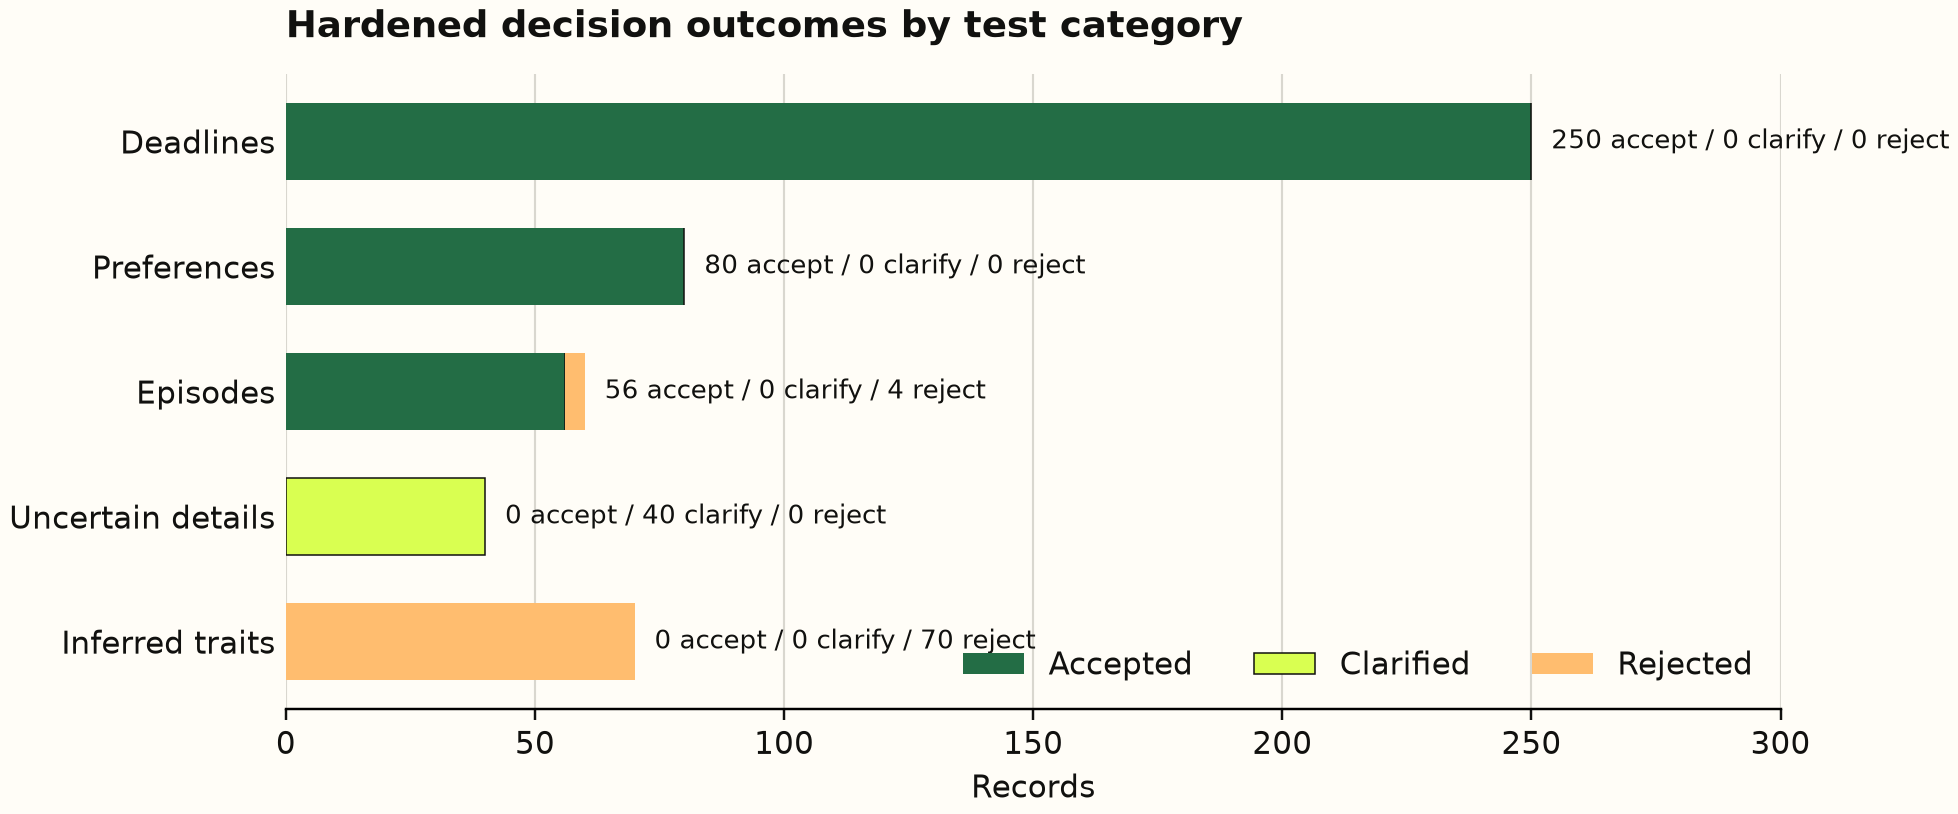
\includegraphics[width=\textwidth]{figures/category_outcomes.png}\end{center}
\clearpage
\section*{Detailed category table}
\begin{center}\begin{tabular}{lrrrr}\toprule
Category & Accept & Clarify & Reject & Expected decision\\\midrule
Explicit deadlines & 250 & 0 & 0 & Accept\\
Explicit preferences & 80 & 0 & 0 & Accept\\
Explicit episodes & 56 & 0 & 4 & Accept\\
Uncertain details & 0 & 40 & 0 & Clarify\\
Inferred traits & 0 & 0 & 70 & Reject\\\bottomrule
\end{tabular}\end{center}
\begin{center}
\begin{tabular}{cc}
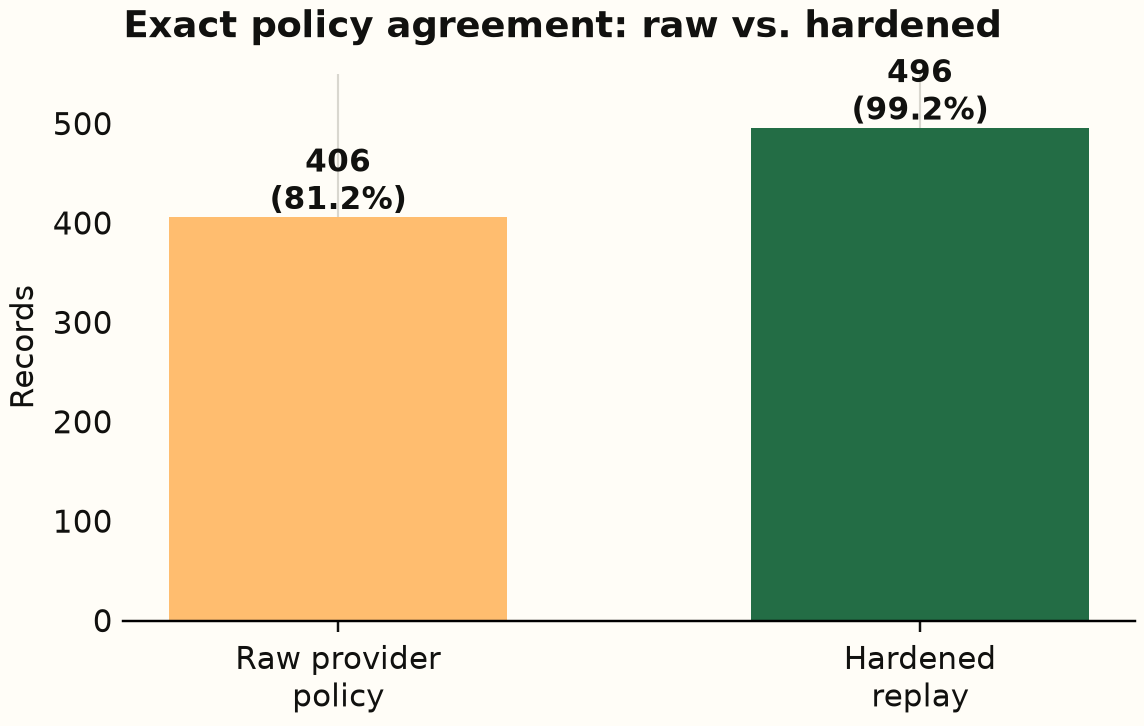
\includegraphics[width=.47\textwidth]{figures/policy_match.png} &
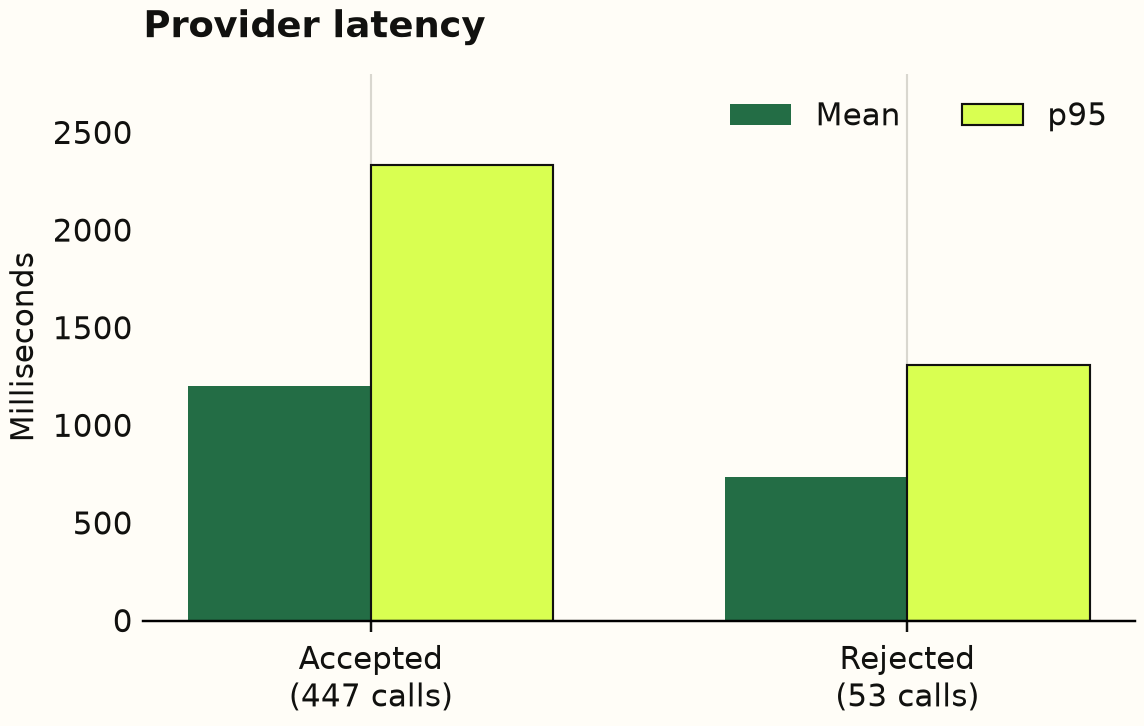
\includegraphics[width=.47\textwidth]{figures/latency_comparison.png}
\end{tabular}
\end{center}
\section*{Interpretation and action}
The source-boundary layer deliberately outranks provider classification when the person says they are uncertain or explicitly rejects a personal label. It also rejects non-verbatim evidence before persistence. This changes the raw provider's 50 false inferred-trait acceptances into rejections and makes all 40 uncertainty cases visible as clarification. Four explicit episode prompts still fail because Sarvam produced no acceptable explicit candidate or marked one as non-explicit; these remain visible failures rather than being promoted automatically.
\begin{enumerate}
  \item Keep the source-boundary regressions for explicit negations, uncertainty, and non-verbatim evidence.
  \item Improve the extraction prompt for explicit episodes, then rerun the stored corpus as a new provider audit.
  \item Preserve the four failing episode records as adversarial tests; do not patch them into acceptance without evidence.
\end{enumerate}
\section*{Audit and reproducibility}
The raw provider audit is persisted locally in \texttt{provider\_evaluation\_runs} and \texttt{provider\_evaluation\_records}. The \texttt{eval:provider-replay} command replays it into an isolated audit scope and writes a machine-readable end-to-end report. No provider rerun is needed for later analysis.
\end{document}
